In this phase we have defined the review protocol. This protocol contains: (\textit{i}) the research questions, (\textit{ii}) the search strategy, (\textit{iii}) the inclusion and exclusion criteria and (\textit{iv}) the data extraction and synthesis method.

Research questions must embody the review study purpose. Moreover, these questions reflect the general scope of the review study. The scope is comprised of population (i.e., population group observed by the intervention), intervention (i.e., what is going to be observed in the context of the planned review study), and outcomes of relevance (i.e., the results of the intervention). Furthermore, during the conduction of this step, it was also necessary to establish the scope of the review study. According to the systematic review process~\cite{Kitchenham}, the scope has to be established using the PICO criteria. Thus, herein our \textbf{Population} is published scientific literature reporting on some existing mining technique for crosscutting concerns. The \textbf{Intervention} is published scientific literature interested with mining technique for crosscutting concerns. The \textbf{Comparison} is not applied herein. Finally, the \textbf{Outcomes of relevance} is an overview of the studies that have been conducted in the field of crosscutting concern mining, emphasizing primary studies that report on the techniques used in the research area, from observing such an aggregated data set, we also intend to provide insight into the frequencies of publication over time to inspect trends.   

%\begin{itemize}

%\item \textbf{Population:} published scientific literature reporting on some existing mining techniques for crosscutting concern.

%\item \textbf{Intervention:} published scientific literature concerned with mining techniques for crosscutting concern. Furthermore, we also aim at determining which techniques are the most used within academic settings.

%\item \textbf{Comparison:} No applied herein.

%\item \textbf{Outcomes of relevance:} an overview of the studies that have been conducted in the field of crosscutting concern mining, emphasizing primary studies that report on the techniques used in the research area. From observing such an aggregated data set we also intend to provide insight into the frequencies of publication over time to inspect trends.

%\end{itemize} 

As described before, the objective of this review is to find out \textbf{which techniques are employed in mining techniques for crosscutting concerns. Moreover, we intent to extend the the taxonomy presented by Kellens et al.~\cite{Kellens}. Finally, we also want to recommend possible combination of the identified techniques in order to identify remaining open research questions and possible avenues for future research}. In order to achieve such objectives we worked out five research questions. The questions are:

\begin{description}

\item[\textbf{RQ$_1$:}] What are the mining techniques that are currently explored in the literature?

\item[\textbf{RQ$_2$:}]  Which assessment techniques have been employed to evaluate these techniques and what are the results for common concerns?

\item[\textbf{RQ$_3$:}]  Is there any difference in the precision and recall metrics when different techniques are used for mining the same concern?

\item[\textbf{RQ$_4$:}] Given a set of concerns, which are the most indicated techniques for performing the mining?

\item[\textbf{RQ$_5$:}] How can someone combine the techniques for improving the precision and recall metrics?

%\item[\textbf{RQ$_3$:}]  Considering the techniques that we found, which ones have automated support?

\end{description}

Afterwards, we have defined the search string and chosen the electronic databases. The search string was created based upon the following keywords: \textit{approach, method, technique, methodology, aspect oriented, aspect-oriented, aspect mining, concern mining, coding mining, code mining, crosscutting concerns, cross-cutting concerns, Separation of Concern, SoC}. A sophisticated search string was constructed using boolean operators i.e., \textit{AND}, \textit{OR} and \textit{NOT}. Figure~\ref{search_string} shows the search string elaborated. The search have encompassed electronic databases which are deemed as the most relevant scientific sources~\cite{Dyba} and therefore likely to contain important primary studies. We have used the search string on the following electronic databases: \textit{ACM} (portal.acm.org), \textit{IEEE} (ieeexplore.ieee.org), \textit{Scopus} (scopus.com) and \textit{Springer} (springer.com/lncs). %Furthermore, no limits were placed on date of publication with a view to not restrict the review study scope. %Aimed at keeping track of the selected papers, we used JabRef\footnote{http://jabref.sourceforge.net/}, an open source system for bibliography reference management. 

\begin{figure}[!h]
\centering
  % Requires \usepackage{graphicx}
  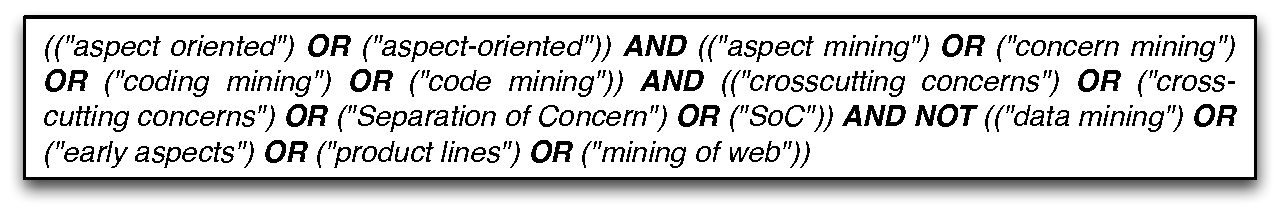
\includegraphics[scale=0.35]{figuras/search_string}
\caption{Search String.}
\label{search_string}
\end{figure} 

Then, in order to determine which primary studies are relevant to answer our research questions, we have applied a set of inclusion and exclusion criteria. Inclusion criteria devised and applied are:

\begin{enumerate}[(a)]%for small alpha-characters within brackets.
\item \textbf{The primary study presents at least one mining technique for crosscutting concern:} the encountered techniques must assist the software engineer in the crosscutting concern mining.
\item \textbf{The primary study presents at least one type of evaluation technique for mining techniques for crosscutting concern:} without the results of the evaluation we neither would be able to make comparisons desired nor would we propose a set of combination of the identified techniques. 
%\textbf{IC$_1$:} the primary study presents at least one mining technique for crosscutting concern
\end{enumerate}

Not all of these criteria must be present for every primary study. However, at least the former (a) must be present. If all criteria were mandatory, the number of selected techniques would decrease significantly.

Exclusion criteria devised and applied are:
\begin{enumerate}[(a)]
\item \textbf{The primary study presents data mining technique. Nevertheless, such technique is applied to databases and not for crosscutting concern mining:} techniques which are applied to databases were not included, since this sort of techniques is outside the scope of this paper.
\item \textbf{The primary study is a short paper:} papers with two pages or less were not considered herein, since we considered that this kind of study do not own sufficient information. 
\end{enumerate}

% \textbf{IC$_1$:} the primary study presents at least one mining technique for crosscutting concern and \textbf{IC$_2$:} the primary study presents at least one type of evaluation technique for crosscutting concern. And the following exclusion criteria: \textbf{EC$_1$:} the primary study presents data mining technique, however, such technique is applied to databases and not for crosscutting concern mining and \textbf{EC$_2$:} the primary study is a short paper (papers with twos pages or less).

%\begin{description}

%\item[\textbf{IC$_1$:}] The primary study presents at least one mining technique for crosscutting concern

%\item[\textbf{IC$_2$:}] The primary study presents at least one type of evaluation technique for crosscutting concern.

%\end{description}

%and the following exclusion criteria:

%\begin{description}

%\item[\textbf{EC$_1$:}] The primary study is not about mining techniques for crosscutting concern.

%\item[\textbf{EC$_2$:}] The primary study presents data mining technique. However, such technique is applied to databases and not for crosscutting concern mining.

%\item[\textbf{EC$_3$:}] The primary study is not available in an electronic format.

%\item[\textbf{EC$_3$:}] The primary study is a short paper (papers with twos pages or less).

%\item[\textbf{EC$_5$:}] The primary study is written neither english nor portuguese.

%\end{description}

We devised data extraction forms to accurately record the information obtained by the researchers from the primary studies. The form for data extraction provides some standard information, such as (\textit{i}) name of the techniques identified, (\textit{ii}) date of data extraction, (\textit{iii}) title, authors, journal, publication details and (\textit{iv}) a list of each conclusion and statement encountered for each sub-question. 

During the extraction process, the data of each primary study were independently gathered by two reviewers. The review was performed in August, 2012 by a M.Sc. and a Ph.D. students; the achieved results were crossed and then validated. All the results of the search process are documented in the web material\footnote{http://tinyurl.com/99spmaz}. Therefore, it is clear to others how thorough the search was, and how they can find the same documents.
